\chapter{UJI COBA DAN EVALUASI}

Pada bab ini dijelaskan tentang uji coba dan evaluasi dari implementasi yang telah dilakukan pada tugas akhir ini.

\section{Lingkungan Uji Coba}

Linkungan uji coba yang digunakan adalah salah satu sistem yang digunakan situs penilaian daring SPOJ, yaitu kluster \textit{Cube} dengan spesifikasi sebagai berikut:

\begin{enumerate}
	\item Perangkat Keras:
	\begin{itemize}
		\item \textit{Processor} Intel(R) Pentium G860 CPU @ 3GHz.
		\item \textit{Memory} 1536 MB.
	\end{itemize}
	\item Perangkat Lunak:
	\begin{itemize}
		\item \textit{Compiler} CPP14.
	\end{itemize}			
\end{enumerate} 

\section{Uji Coba Kebenaran}

Uji coba kebenaran dilakukan dengan mengirimkan kode sumber program ke dalam situs penilaian daring SPOJ dan melakukan hasil uji coba kasus sederhana dengan langkah-langkah sesuai dengan algoritma yang telah dirancang dengan keluaran sistem. Permasalahan yang diselesaikan adalah \textit{The Bytelandian Cryptographer (Act IV)}. Hasil uji coba dengan waktu terbaik pada situs SPOJ ditunjukkan pada Gambar \ref{fig:best_submission}.

Selain itu, dilakukan pengujian sebanyak 30 kali pada situs penilaian daring SPOJ untuk melihat variasi waktu dan memori  yang dibutuhkan program. Hasil uji coba sebanyak 30 kali dapat dilihat pada Gambar \ref{fig:submission1}, \ref{fig:submission2}.

Dari hasil uji coba pada Gambar \ref{fig:submission1} dan \ref{fig:submission2}, dapat disederhanakan menjadi Gambar \ref{fig:chart}. Dari informasi yang terdapat pada Gambar \ref{fig:chart} dapat ditarik beberapa informasi seperti yang tertera pada Tabel \ref{tab:statistik}.

\begin{table}[H]
	\centering
	\caption{Kecepatan Maksimal, Minimal, dan Rata-Rata dari Hasil Uji Coba Pengumpulan 30 Kali pada Situs Pengujian Daring Spoj}
	\begin{tabular}{|l|l|} \hline
		Waktu Maksimal & $ 4,49 $ detik\\ \hline
		Waktu Minimal & $ 4,38 $ detik\\ \hline
		Waktu Rata-Rata & $ 4.418 $ detik\\ \hline
		Memori Maksimal & $ 27 $ MB\\ \hline
		Memori Minimal & $ 26 $ MB\\ \hline
		Memori Rata-Rata & $ 26.5 $ MB\\ \hline
	\end{tabular}
	\label{tab:statistik}
\end{table}

\indent Berdasarkan Tabel \ref{tab:statistik} didapatkan waktu eksekusi rata-rata $ 4.418 $ detik dan waktu maksimal $ 4,47 $ detik. Waktu eksekusi tersebut $3,8$ kali lebih cepat dari batas waktu eksekusi yang tertera pada deskripsi permasalahan, yaitu $ 17 $ detik.


\indent Uji Coba dengan menggunakan contoh kasus uji coba yang tersedia di dalam SPOJ \textit{The Bytelandian Cryptographer (Act IV)}. Sebagai contoh akan digunakan kasus ujicoba yang menggunakan baik mencari panjang kunci maupun \textit{intersection} yang terjadi dalam permasalahan ini.


\indent Sesuai dengan algoritma yang telah dirancang pada \textit{pseudocode} yang terdapat pada Gambar \ref{fig:solvefx1} dan \ref{fig:solvefx2} maupun pada Gambar \ref{fig:validity}. Algoritma ini akan melakukan perulangan yang terdapat pada \plaintext dan \ciphertext yang diperoleh dari inputan dan akan menyimpan posisi karakter dengan ketentuan apabila pada indeks tersebut diketahui baik \plaintext dan \ciphertext beserta dengan selisih antara \ciphertext dan \plaintext. Selanjutnya juga menyimpan posisi karakter yang diperoleh dari \ciphertext dengan ketentuan apabila \ciphertext pada indeks tersebut diketahui karakternya dan \plaintext diindeks tersebut tidak diketahui karakternya. Misalnya diambilkan contoh dari Tabel \ref{tab:contoh3}. Maka yang disimpan untuk bagian yang diketahui keduanya adalah indeks ke 1 dengan selisih 0 dan indeks ke 2 dengan selisih 0, sedangkan untuk yang disimpan pada diketahui \ciphertext saja maka jawabannya semua indeks kecual indeks ke 1 dan 2. Selanjutnya, akan membandingkan antara panjang \plaintext atau \ciphertext dengan $m$ untuk dicari yang lebih kecil yang mana. Selanjutnya, mulai mengiterasi panjang kunci yang akan muncul dari $\frac{m}{2}+1$ sampai dengan $m$. Didalam iterasi tersebut akan dilakukan pengecekan apakah nilai $m$ dengan fungsi VALIDITY($m$). Jika gagal, program akan melanjutkan untuk mencari panjang kunci selanjutnya, sebaliknya jika hasil dari fungsi tersebut benar maka akan melanjutnya proses \textit{generate} hasil yang telah diperoleh dari panjang kunci secara satu per satu dan dibandingan dengan hasil yang sudah ada sebelumnya. Perbandingan tersebut akan mengikuti aturan apabila suatu indeks ternyata ada yang konflik, baik yang nilainya berubah ataupun tidak memiliki suatu aturan kunci dari panjang kunci yang saat itu tersedia. Maka, hasil dari indeks tersebut adalah "*" dan menghapus elemen dari tempat penyimpanan yang menampung indeks \plaintext yang "*" dan \ciphertext yang tidak "*". Apabila tidak ada konflik maka \plaintext pada indeks tersebut tidak menjadi "*". Seperti contohnya terdapat pada Tabel \ref{tab:contoh2} dan Tabel \ref{tab:contoh3}  


\indent Sehingga hasil keluaran yang diperoleh dari algoritma ini adalah seluruh \plaintext yang dapat dibentuk.

\section{Analisa Kompleksitas Waktu}
Pada \textit{pseudocode} yang terdapat pada Gambar \ref{fig:mainfx}. Untuk setiap kasus ujicoba terdapat 2 fungsi utama. Dengan menggunakan \textit{Kasiski Examination} dan \textit{Intersection} yang terdapat pada fungsi SOLVE dan VALIDITY memiliki kompleksitas $\mathcal{O}((n+(\frac{M}{2}*(N+S))))$. $n$ adalah panjang karakter \plaintext atau \textit{ciphertext}, $M/2$ adalah batas atas kunci dibagi dengan 2, $N$ adalah jumlah posisi karakter yang terdapat bisa jadi memiliki suatu nilai yang bisa didapat dari \textit{ciphertext}, dan $S$ adalah jumlah posisi karakter yang diketahui. Untuk kompleksitas fungsi VALIDITY $\mathcal{O}(S)$. Sehingga kompleksitas dapat disederhanakan menjadi $\mathcal{O}(T*\frac{M}{2}*(N+S))$.
\indent Sehingga secara keseluruhan kompleksitas dari algoritma yang dirancang pada tugas akhir ini adalah $\mathcal{O}(T*\frac{M}{2}*(N+S))$.

Pada umumnya, eksekusi program pada situs penilaian daring SPOJ adalah $ 1 $ detik untuk setiap $ 1.000.000.000 $ proses. Ekseskusi program dengan kompleksitas $\mathcal{O}(T*\frac{M}{2}*(N+S))$. Pada \textit{worst case} $T*(N+S)=1.000.000$, sedangkan $\frac{M}{2}$ adalah $50.000$. Hasilnya melebihi dari 50 miliar perulangan, maka waktu yang dibutuhkan adalah 50 detik. Jika hal ini terjadi maka waktu eksekusi akan berjalan dengan sangat lama. Estimasi waktu kurang lebih $100$ detik, tetapi kenyataan yang terjadi tidak demikian, alasannya karena jumlah $S$ bisa berkurang seiring dengan perulangan yang ada.
\\
Sebagai perbandingan ujicoba kinerja antara menggunakan algoritma \textit{Naive} dan algoritma optimasi \textit{Kasiski Examination} dengan \textit{Intersection}, dapat dilihat pada Gambar \ref{fig:banding12}. Maka, dapat ditarik kesimpulan bahwa algoritma optimasi \textit{Kasiski Examination} dengan \textit{Intersection} jauh lebih cepat dibandingan algoritma \textit{Naive}.
%dengan batas atas panjang kunci yang uniform yaitu 41 dan struktur plaintext dan cipher yang berulang. sehingga dapat memperlihat pergerakan waktu sesungguhnya yang dibutuhkan. ini hanyalah sebagian kecil dari proses program yang telah dijalankan. dengan algoritma naive pasti TLE. naive itu menggunakan sama persis dengan kasiski examination dan intersection tetapi bedanya dimana kalau yg optimasi ada prunningnya sedangkan yang naive tanpa pruning apapun.
	
	\begin{figure}[H]
	\centering
  	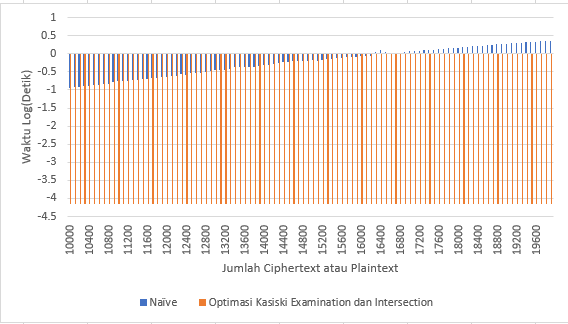
\includegraphics[scale=0.7]{images/bab5/ACD.png}
  	\caption{Gambar Perbandingan Kinerja Algoritma Optimasi \textit{Kasiski Examination} dengan \textit{Intersection} dan \textit{Intersection}}
  	\label{fig:banding12}
	\end{figure}
	
	
%telah dilakukan ujicoba apabila menggunakan pure n2 maka tidak akan memungkinkan untuk menyelesaikan masalah ini dengan cepat dan tidak akan berhasil. dilakukan juga untuk membuat perubahan pada intersection akan tetapi juga sesuatu kegagalan. perubahan yang dilakukan untuk mengubah struktur data harus mengakses dengan cepat hanya hal yang mungkin, tapi ini sudah dilakukan . maka yang paling mungkin adalah melakukan optimasi pada pencarian panjang kunci. uji yang telah dilakukan degan menggunakan bilangan prima -> gagal. dengan pigeonhole juga gagal. apbila n=m -> meh podo ae. 